\documentclass[conference]{IEEEtran}
\IEEEoverridecommandlockouts
\usepackage{cite}
\usepackage{amsmath,amssymb,amsfonts}
\usepackage{algorithmic}
\usepackage{graphicx}
\usepackage{textcomp}
\usepackage{xcolor}
\usepackage{booktabs}
\def\BibTeX{{\rm B\kern-.05em{\sc i\kern-.025em b}\kern-.08em
    T\kern-.1667em\lower.7ex\hbox{E}\kern-.125emX}}

\begin{document}

\title{Determinants of Household Participation in Securities Markets: An Empirical Analysis\\
\thanks{Based on the 2025 SEBI Household Survey on Securities Market Participation.}
}

\author{\IEEEauthorblockN{Shivansh Verma}
\IEEEauthorblockA{\textit{Dept of CS} \\
\textit{Ashoka University}\\
Sonipat, India \\
shivansh.verma\_ug2023@ashoka.edu.in}
\and
\IEEEauthorblockN{Sashwat Dhanuka}
\IEEEauthorblockA{\textit{Dept of CS} \\
\textit{Ashoka University}\\
Sonipat, India \\
sashwat.dhanuka\_ug2023@ashoka.edu.in}
}

\maketitle

\begin{abstract}
Household participation in capital markets is a crucial driver of financial inclusion and wealth creation, yet it remains disproportionately skewed across demographic lines. Using a large-scale micro-dataset from the 2025 SEBI Household Survey ($N=109,430$), this paper empirically analyzes the determinants of securities market participation in India. We employ a logistic regression framework to isolate the socioeconomic drivers of investment, revealing that education and income are the strongest predictors (odds ratios of 1.83 and 1.80, respectively). We further investigate structural barriers deterring non-investors, identifying loss aversion and information asymmetry as primary friction points. To deepen our behavioral insights, we expose a stark Dunning-Kruger effect among overconfident retail traders and measure the impact of ``finfluencers'' on high-risk asset adoption. Finally, we implement Gradient Boosting Classifiers to predict participation, asset choice, and investment horizons based on basic demographic and behavioral metrics. Our predictive models achieve strong discriminatory power for baseline participation (AUC=0.76) and asset allocation (AUC=0.83), validating that while market entry is structurally gated, post-entry behavior is heavily dictated by psychographic traits and financial literacy.
\end{abstract}

\begin{IEEEkeywords}
Financial Inclusion, Securities Markets, Household Finance, Behavioral Economics, Predictive Modeling
\end{IEEEkeywords}

\section{Introduction}
The democratization of capital markets is essential for broad-based economic growth and household wealth accumulation. In emerging economies like India, retail participation in securities has witnessed a significant surge, catalyzed by digitization and the proliferation of zero-commission trading platforms. Despite this growth, participation remains highly heterogeneous. 

Understanding the determinants of household participation is a central problem in financial economics. Why do certain households allocate capital to mutual funds and equities, while others restrict their savings to traditional, low-yield instruments like fixed deposits? The literature points to a combination of background risk, financial literacy, and trust in institutions. However, most existing studies rely on older data that predate the post-pandemic retail boom, the widespread adoption of digital KYC, and the systemic rise of social media financial influencers.

This paper addresses this gap by utilizing the comprehensive 2025 SEBI Household Survey. We pose four core research questions: (1) Who is likely to participate in the securities market? (2) What structural and behavioral barriers keep the majority of households out? (3) Which securities do participating households prefer, and for how long? and (4) Can we predict these outcomes given basic demographic and behavioral metrics?

The remainder of the paper is organized as follows: Section II details the dataset and methodology. Section III presents the empirical findings regarding determinants, behavioral anomalies, and securities preferences. Section IV details our predictive modeling framework. Finally, Section V concludes with highly condensed policy implications.

\section{Data and Methodology}
\subsection{Dataset}
We utilize micro-data from the 2025 SEBI Household Survey on Securities Market Participation, comprising a nationally representative sample of 109,430 households across India. The dataset captures detailed demographic variables (age, gender, education, income), geographical data, and behavioral metrics (risk tolerance, market perception). Crucially, the survey differentiates between \textit{investors} (25.5\%) and \textit{non-investors} (74.5\%).

\subsection{Econometric \& Predictive Specification}
To identify the core determinants of participation, we first estimate a binary logistic regression model where the dependent variable is active investment status ($Y_i \in \{0,1\}$). Independent variables are normalized to extract comparable odds ratios.

To expand this into a forecasting paradigm, we utilize Histogram-based Gradient Boosting Classifiers to predict three distinct outcomes: (Model 1) the binary likelihood of participation; (Model 2) the choice between market-linked securities (Equity/MF) vs. traditional instruments; and (Model 3) the propensity to hold equity for the long-term.

\section{Empirical Results}

\subsection{Determinants of Participation \& Overconfidence}
The results of the logistic regression demonstrate a stark divide driven by human and financial capital. As depicted in Fig. \ref{fig:odds_ratios}, education and income emerge as the strongest statistical determinants. A one-standard-deviation increase in years of education increases the odds of market participation by 1.83 times, holding other factors constant. Similarly, the odds ratio for log-income is 1.80. Urban residency (OR=1.56) and male gender (OR=1.56) also play significant roles, highlighting systemic geographical and gender-based disparities.

\begin{figure}[htbp]
\centerline{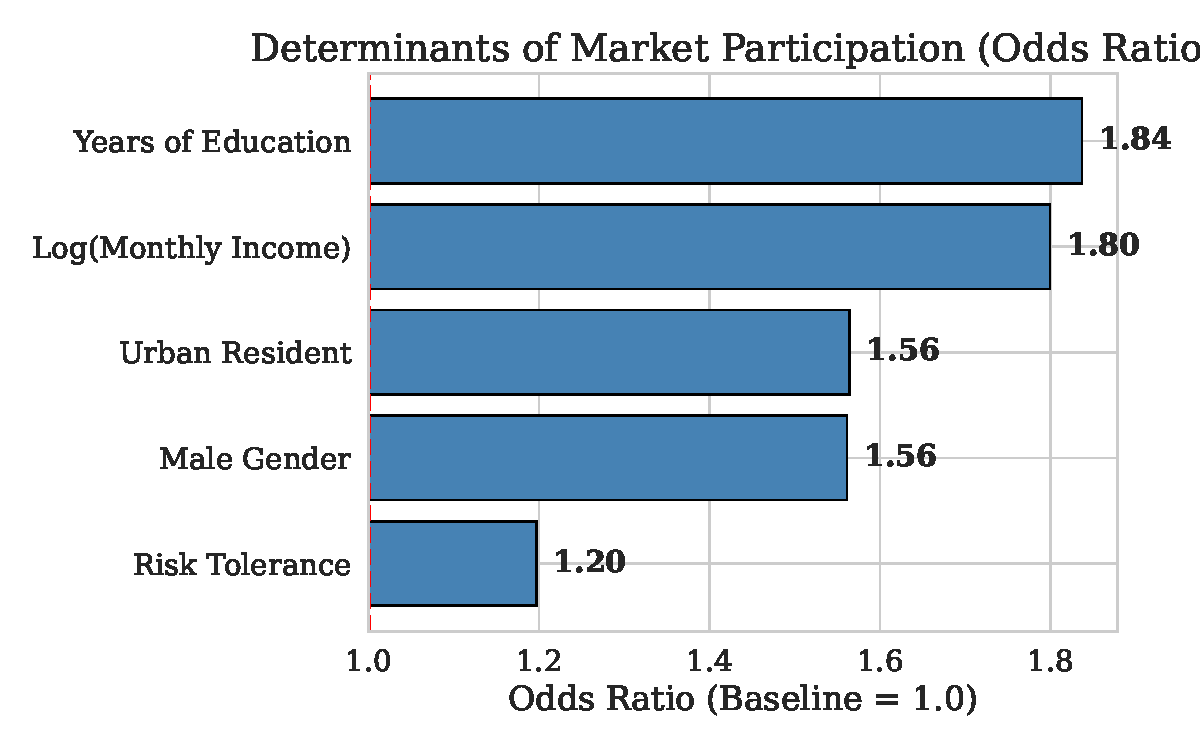
\includegraphics[width=\linewidth]{../figures/fig1_odds_ratios.pdf}}
\caption{Forest plot of Odds Ratios for determinants of market participation. Baseline is 1.0. Education and income show the highest predictive power.}
\label{fig:odds_ratios}
\end{figure}

For the 74.5\% of households that remain completely outside the securities market, self-reported barriers (Fig. \ref{fig:barriers}) indicate that behavioral frictions dominate structural ones. Specifically, ``Fear of Loss'' is the top barrier, closely followed by ``Lack of Knowledge'' and ``Lack of Trust''. This suggests that while digital platforms have solved access friction, the cognitive and emotional friction of investing remains high.

\begin{figure}[htbp]
\centerline{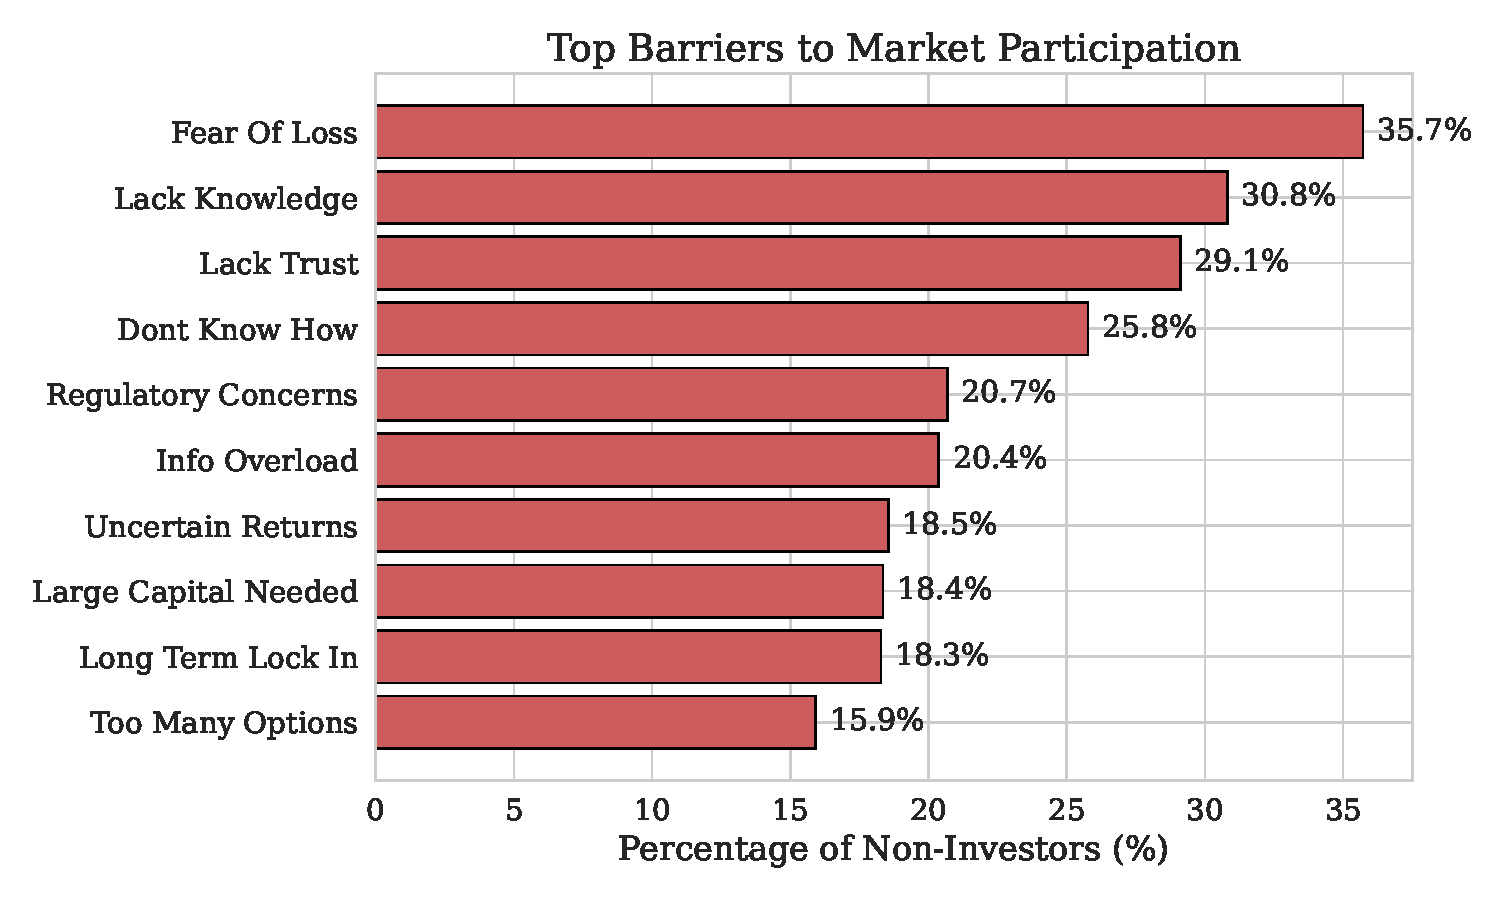
\includegraphics[width=\linewidth]{../figures/fig2_barriers.pdf}}
\caption{Top barriers cited by non-investors. Loss aversion and information asymmetry (lack of knowledge/trust) are the primary deterrents.}
\label{fig:barriers}
\end{figure}

Diving deeper into the ``Knowledge'' barrier, we analyzed the divergence between self-reported market familiarity and actual scores on an objective financial literacy quiz. We discovered a profound Dunning-Kruger effect: investors who are ``overconfident'' (high perceived familiarity, low actual knowledge) are disproportionately likely to hold high-risk assets like Futures \& Options (F\&O) and Cryptocurrency compared to calibrated investors (Fig. \ref{fig:dunning_kruger}). This behavioral anomaly underscores why traditional models of rational participation often fail to capture modern retail dynamics.

\begin{figure}[htbp]
\centerline{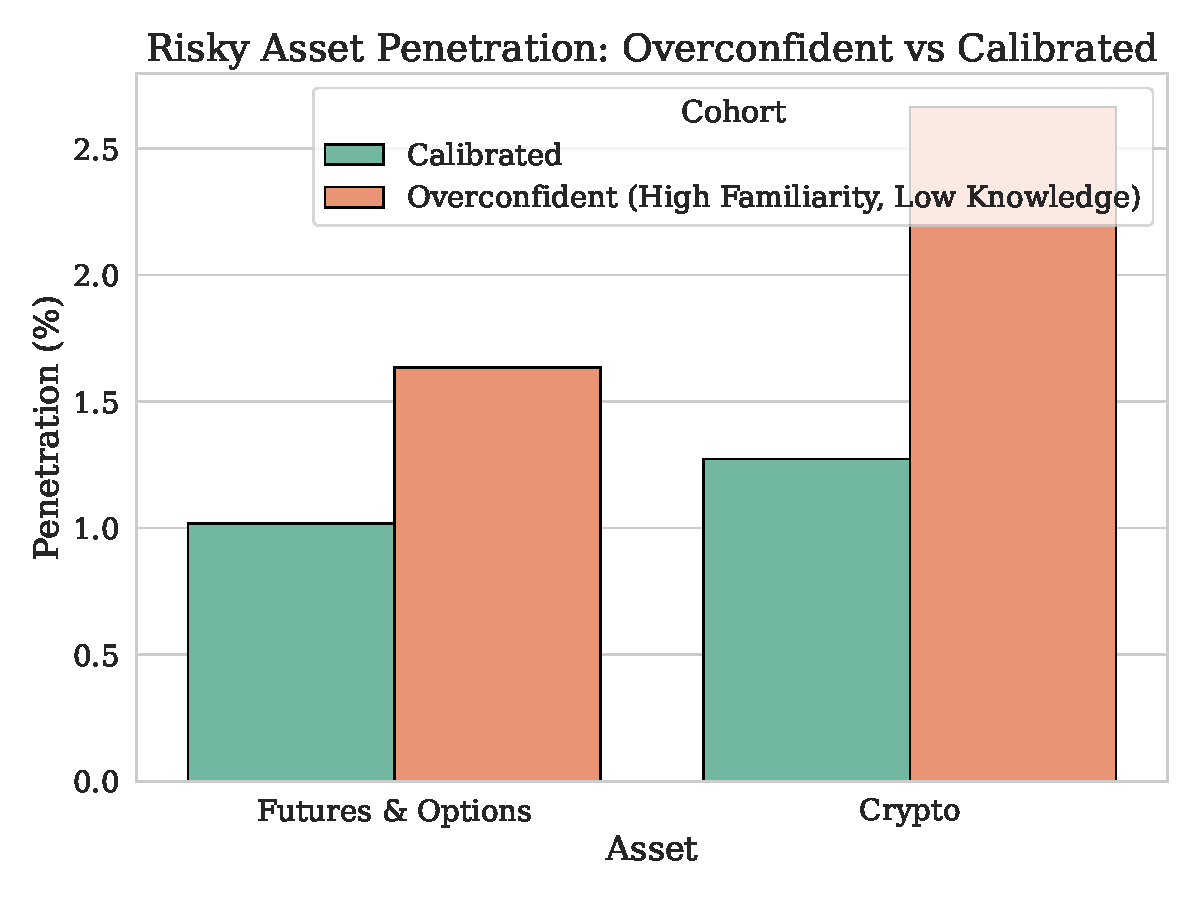
\includegraphics[width=\linewidth]{../figures/fig5_dunning_kruger.pdf}}
\caption{Risky Asset Penetration. Overconfident investors participate in highly speculative assets at significantly higher rates than calibrated investors.}
\label{fig:dunning_kruger}
\end{figure}

\subsection{Securities Preferences, Demographics, and Influencers}
Once households overcome the barrier to entry, their product preferences shift dynamically with income. Fig. \ref{fig:securities_income} illustrates the penetration of various financial instruments across income quartiles. Fixed Deposits (FDs) remain the bedrock of Indian savings, showing uniformly high penetration. However, the adoption of market-linked securities---specifically Mutual Funds/ETFs and Direct Equity---scales dramatically in the higher income brackets, indicating that risk appetite scales non-linearly with wealth.

\begin{figure}[htbp]
\centerline{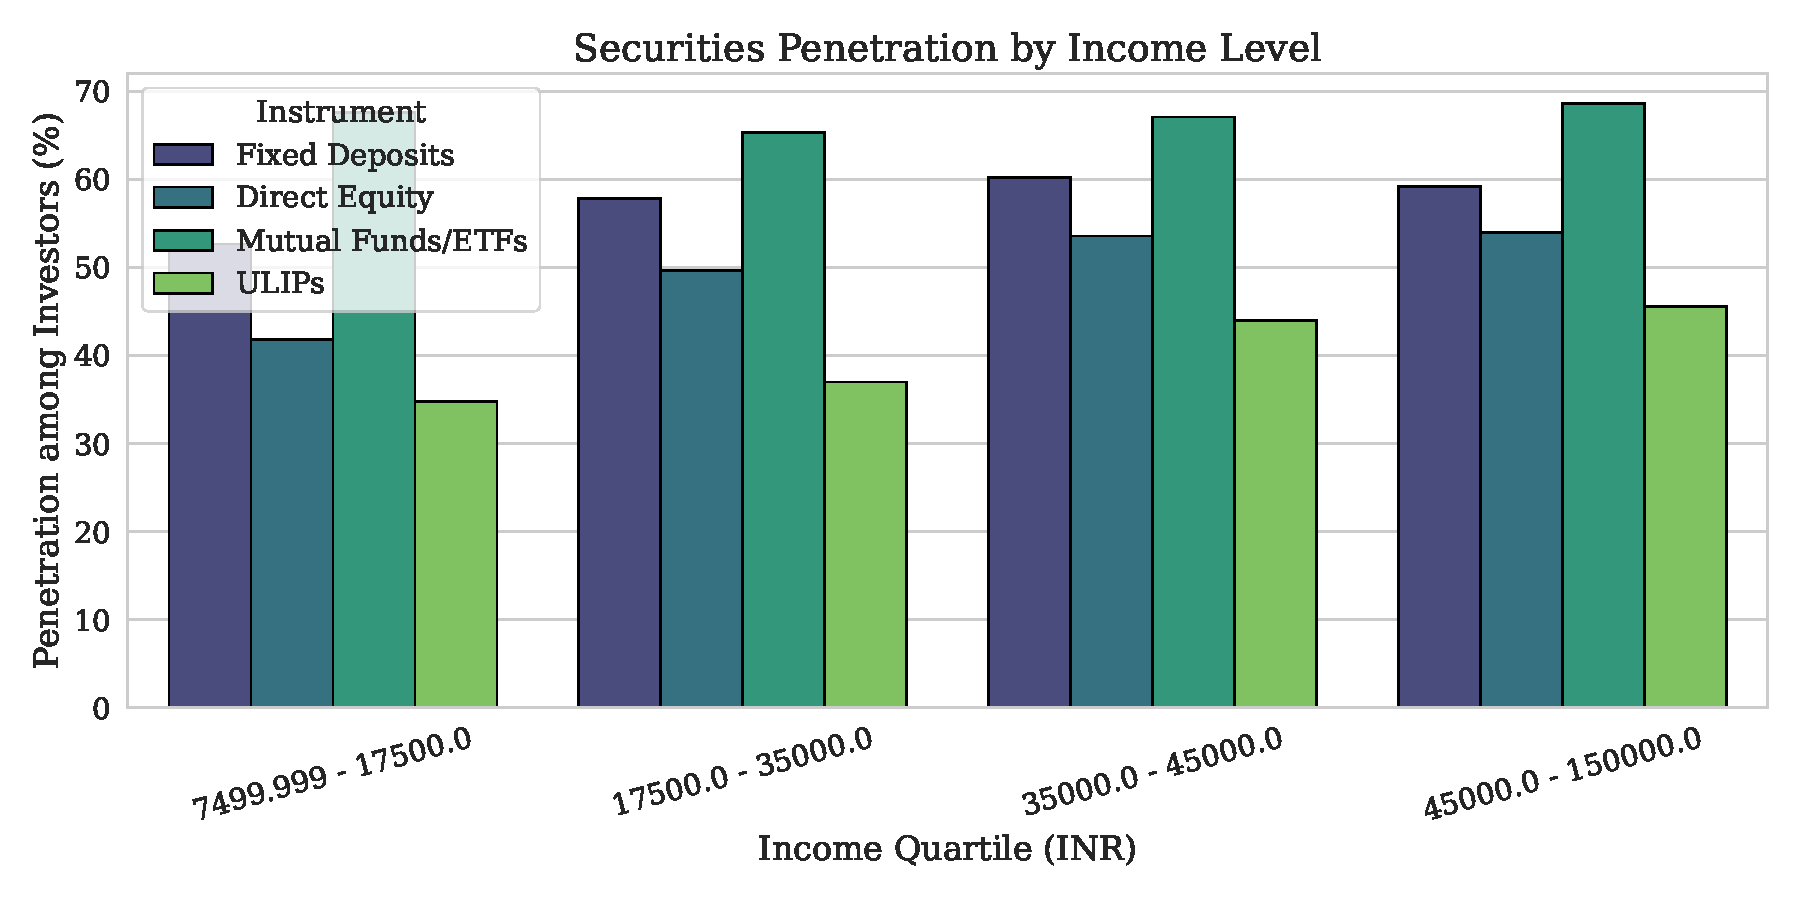
\includegraphics[width=\linewidth]{../figures/fig3_securities_income.pdf}}
\caption{Securities penetration among investors, segmented by income quartile. Market-linked instruments scale sharply with wealth.}
\label{fig:securities_income}
\end{figure}

Crucially, the choice of securities is heavily modulated by where investors source their information. Contrasting investors who rely exclusively on Social Media ``Finfluencers'' against those using traditional Financial Professionals reveals a sharp behavioral divide. As seen in Fig. \ref{fig:finfluencers}, the Finfluencer cohort is primarily motivated by ``Quick Gains,'' whereas the professionally-advised cohort seeks ``Long Term Growth.'' (Prevalence here is calculated as the percentage of investors within a specific information-source cohort who selected a given motive). This ties directly to the overconfidence trap discussed earlier, painting a picture of a segmented market where information source dictates risk behavior.

\begin{figure}[htbp]
\centerline{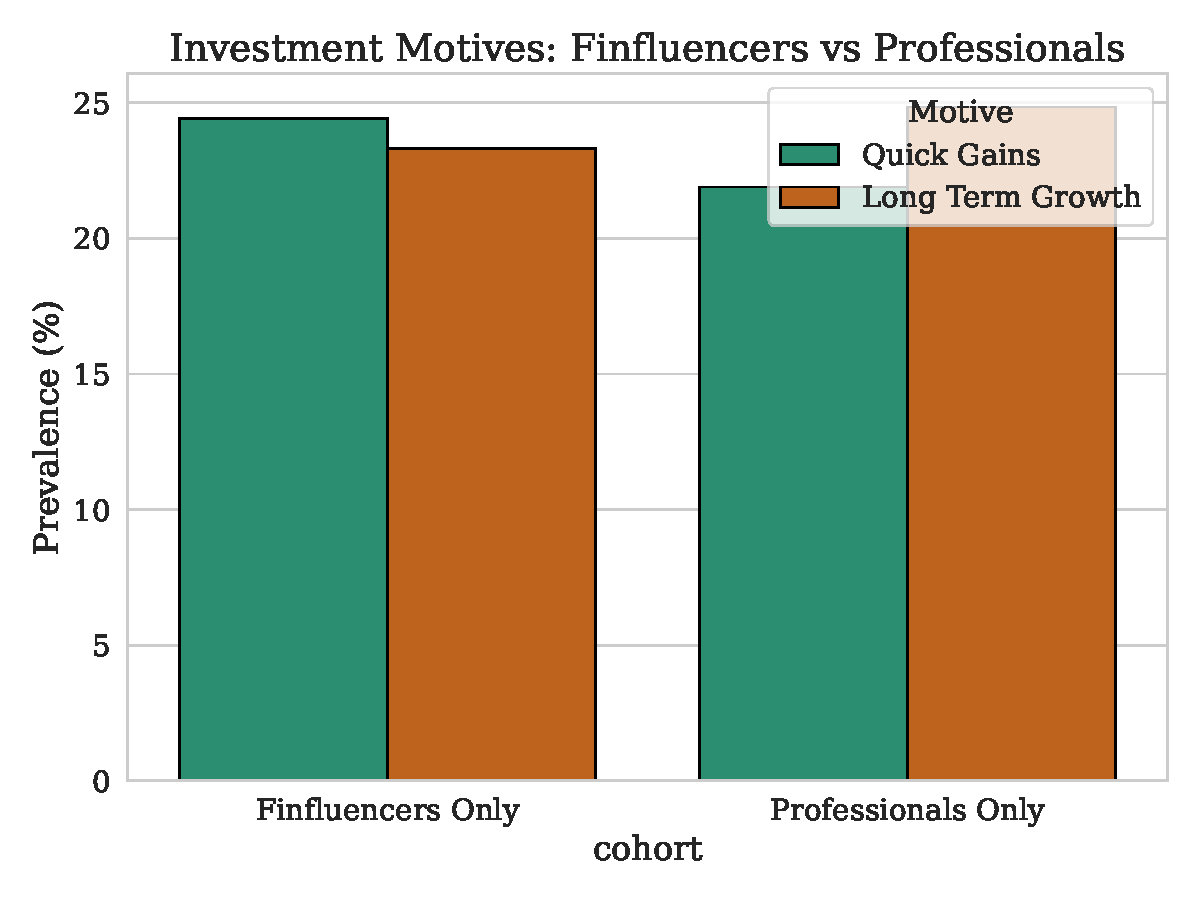
\includegraphics[width=\linewidth]{../figures/fig6_finfluencers.pdf}}
\caption{Investment Motives segmented by Information Source. Prevalence denotes the percentage of investors within each cohort holding a specific motive. Social media heavily biases investors toward short-term speculative gains.}
\label{fig:finfluencers}
\end{figure}

\subsection{Investment Horizons}
Holding duration preferences (Fig. \ref{fig:duration}) challenge the notion that all retail investors are short-term speculators. A significant plurality of equity and mutual fund investors define their holding periods as ``Long term''. In contrast, sophisticated derivative products (F\&O) are predominantly utilized for ``Short term'' horizons, aligning with the motivations of the Finfluencer-driven cohort.

\begin{figure}[htbp]
\centerline{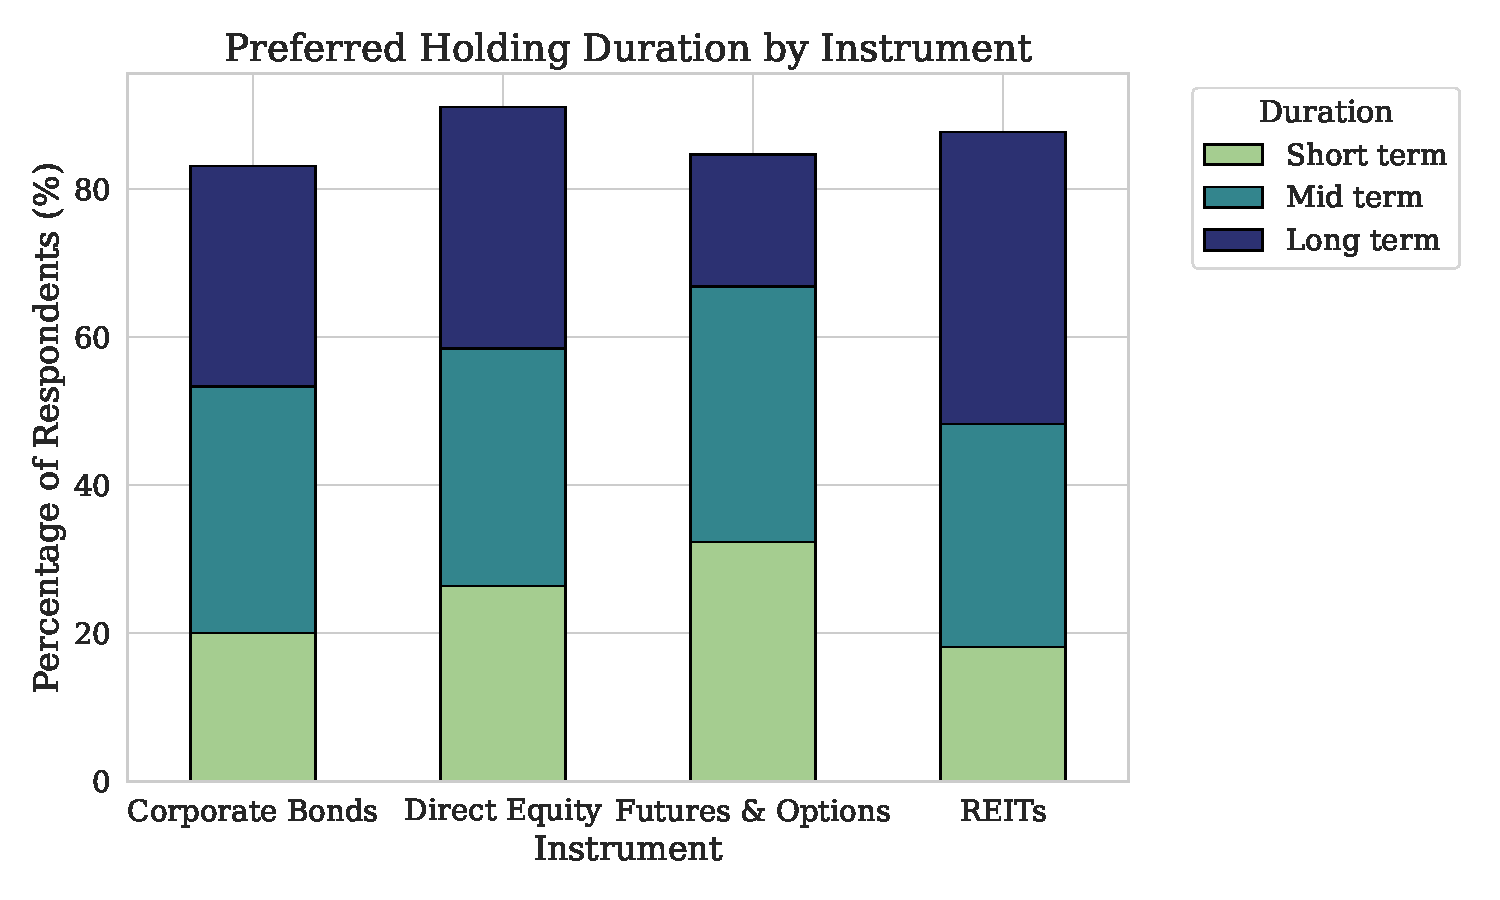
\includegraphics[width=\linewidth]{../figures/fig4_duration.pdf}}
\caption{Preferred holding durations across different asset classes. Direct equities are largely held for the long term, whereas derivatives skew short term.}
\label{fig:duration}
\end{figure}

\section{Predictive Modeling: Forecasting Household Participation}
To operationalize our findings, we utilized Histogram-based Gradient Boosting Classifiers to predict household behavior. Initially, our models relied strictly on basic demographic and risk-tolerance metrics. While this was sufficient to predict baseline participation, it failed to predict post-entry behavior. To resolve this, we expanded the feature space for investor-specific models (Models 2 and 3) to include the behavioral traits uncovered in our earlier analysis.

\begin{figure}[htbp]
\centerline{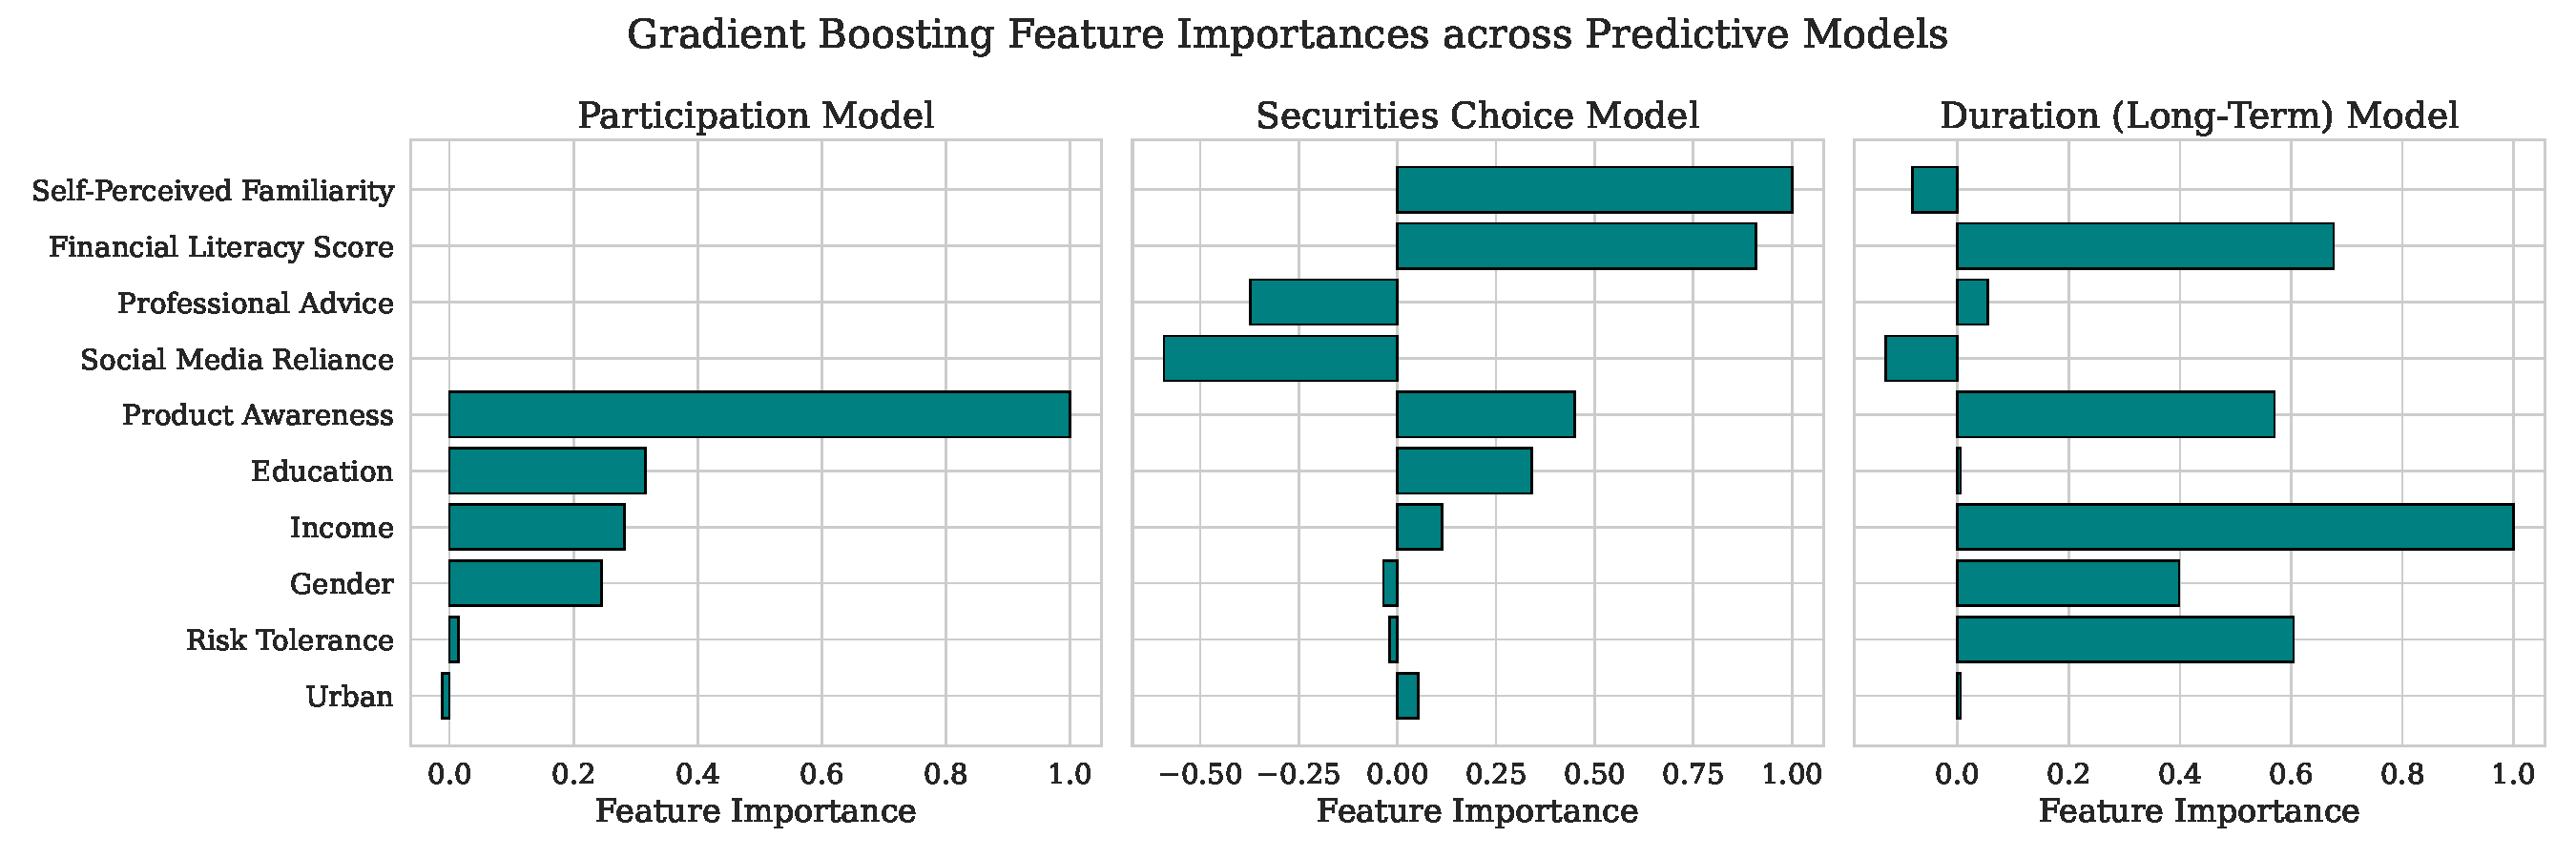
\includegraphics[width=\linewidth]{../figures/fig7_predictive_importance.pdf}}
\caption{Feature Importance across the three Predictive Models. Behavioral features like Familiarity and Financial Literacy heavily dominate the models predicting asset allocation and duration.}
\label{fig:predictive_importance}
\end{figure}

As shown in Fig. \ref{fig:predictive_importance}, injecting behavioral data drastically improves our forecasting capabilities.

\subsection{Model 1: Predicting Participation}
\textbf{Objective:} Predict the binary outcome of whether a household is an active investor ($1$) or a non-investor ($0$). \\
\textbf{Data Fields Used:} Years of Education, Log-transformed Monthly Income, Urban Residency (Binary), Gender (Binary), and Risk Tolerance Preference Score. \\
\textbf{Algorithm \& Split:} HistGradientBoostingClassifier (200 max iterations, balanced class weights) trained on an 80/20 train-test split. \\
\textbf{Performance:} The model achieved an Area Under the Receiver Operating Characteristic Curve (AUC) of 0.76. \\
\textbf{Insight:} Basic metrics are highly effective at predicting \textit{whether} a household will participate. Education and Income heavily dominate the decision boundary, validating that entry is structurally gated.

\subsection{Model 2: Predicting Securities Choice}
\textbf{Objective:} For households that \textit{are} investors, predict if they will hold market-linked securities (Equities or Mutual Funds = $1$) versus sticking exclusively to traditional instruments like Fixed Deposits ($0$). \\
\textbf{Data Fields Used:} All demographic features from Model 1, \textbf{plus} Self-Perceived Stock Market Familiarity, Actual Financial Literacy Score, Social Media Reliance (Binary), and Professional Advice Reliance (Binary). \\
\textbf{Algorithm \& Split:} HistGradientBoostingClassifier trained on an 80/20 train-test split. \\
\textbf{Performance:} The model achieved an impressive AUC of 0.83 (up from 0.60 when using only demographics). \\
\textbf{Insight:} Predicting \textit{how} individuals participate requires behavioral context. Once we include perceived familiarity and objective knowledge, the model's discriminatory power surges.

\subsection{Model 3: Predicting Investment Horizon}
\textbf{Objective:} For equity investors, predict if they will define their holding period as ``Long Term'' ($1$) versus Short/Mid-term ($0$). \\
\textbf{Data Fields Used:} Same extended demographic and behavioral feature set used in Model 2. \\
\textbf{Algorithm \& Split:} HistGradientBoostingClassifier trained on an 80/20 train-test split. \\
\textbf{Performance:} The model achieved an AUC of 0.61 (up from 0.58). \\
\textbf{Insight:} Forecasting \textit{how long} an investor will hold equity remains the hardest prediction task, but injecting information sources and financial literacy provides a measurable improvement over random demographic guessing.

\vspace{0.3cm}
These predictive models validate our core thesis: while structural socioeconomic factors gatekeep entry into the market, post-entry asset allocation and duration are overwhelmingly dictated by psychological factors, financial literacy, and the modern information ecosystem.

\section{Conclusion and Policy Implications}
The 2025 SEBI Household Survey provides compelling evidence that while the Indian securities market is growing, entry remains fundamentally gated by education and income. Once inside the market, however, traditional demographics fail to predict behavior. Instead, a dangerous cocktail of overconfidence and social media influence is driving a subset of retail investors toward highly speculative, short-term derivative trading.

For policymakers, the mandate is clear: interventions must pivot from merely reducing transaction costs to aggressively policing the quality of financial information. Bridging the knowledge gap via targeted, gamified financial literacy programs is essential. Furthermore, the undeniable Dunning-Kruger effect suggests that access to complex derivatives should perhaps be gated by objective literacy tests, rather than self-reported familiarity, to protect the new wave of retail investors from behavioral pitfalls.

\begin{thebibliography}{00}
\bibitem{b1} SEBI, ``Household Survey on Securities Market Participation 2025,'' Securities and Exchange Board of India, 2025.
\end{thebibliography}

\end{document}
